\documentclass[../main.tex]{subfiles}

\begin{document}

\section{Natural Language Tasks and Application}

\begin{itemize}
  \item Machine Translation
  \item Summarization (long text $\rightarrow$ short text)
  \item Dialogue (previous utterance $\rightarrow$ next utterance)
  \item Parsing (input text $\rightarrow$ output parse)
  \item Code generation (natural language $\rightarrow$ Python code)
  \item Entailment
  \item Natural Language Generation
\end{itemize}

\section{Neural Machine Translation}

\begin{itemize}
  \item task of translating a sentence x from one language (source) to a sentence y in another language (target)
  \item (2014) sequence-to-sequence and involves using two RNNs
\end{itemize}

\section{RNN}

\section{Encoder-decoder models}
\begin{itemize}
  \item Conditional Language Model
  \item conditional because predictions are conditioned on the source sentence $x$
  \item Encoder RNN produces an encoding of the source sentence
  \item Decoder RNN is a Language Model generates a target sentence, conditioned on encoding
  \item decoder predicts the next word of the target sentence $y$
  \item "end-to-end", learn entire system with respect to a single loss, optimize the system as a whole, more likely to succeed
  \item Cross entropy loss on probability distribution output from decoder model
  \item Padding short sentences to maximum length of the batch and apply attention mask
  \item Greedy decoding has no way to undo decisions or perform backtracking
  \item Beam search decoding
\end{itemize}

\section{Evaluation Metrics}
\begin{itemize}
  \item BLEU (Bilingual Evaluation Understudy)
  \begin{itemize}
    \item compares machine-written translation to one or several human-written translation and compute a similarity score based on n-gram precision
    \item plus a penalty for too-short translations
    \item useful but imperfect!
  \end{itemize}
\end{itemize}

\section{Challenges}
\begin{itemize}
  \item Out-of-vocabulary words
  \item Domain mismatches between train and test data
  \item Maintaining context over longer text (e.g. translate a whole news article or book)
  \item Low-resource language pairs (e.g. don't have large corpus, language that is not commonly used)
  \item Common sense is hard
  \item Biases in training data (e.g. gender, race, etc)
  \item Models are uninterpretable and do strange things
\end{itemize}



\section{Attention}

\begin{itemize}
  \item Seq-to-seq encodes source sentence into a single embedding vector. This needs to capture all information in the sentence and causes an information bottleneck!
  \item Idea is to encode each word in a sentence into a vector
  \item When decoding, take the linear combination of these vectors weighted by "attention weights"
  \item "Query" vector and "key" vector
  \item Calculate weight for each query-key pair and normalize using softmax to get a probability distribution
  \item Use attention distribution to take weighted sum of encoder hidden states where the weights are the attention scores
  \item Encoder hidden states: $h_{1}, \dotsc, h_{N} \in \mbb{R}^{h}$
  \item Decoder hidden states: $s_{t} \in \mbb{R}^{h}$
  \item Attention scores: $e^{t} = [s_{t}^{T}h_{1}, \dotsc, s_{t}^{T}h_{N}] \in \mbb{R}^{N}$
  \item $\alpha^{t} = \text{softmax}(e^{t}) \in \mbb{R}^{N}$
  \item $a_{t} = \sum_{i=1}^{N} \alpha_{i}^{t}h_{i} \in \mbb{R}^{h}$
  \item Attention allows decoder to focus on certain part of the source
  \item solves the information bottleneck problem and the vanishing gradient problem and more interpretability
  \item we get (soft) alignments for free, never explicitly trained alignment system like Statistical Machine Translation
  \item Given a set of vector values and vector query, attention computes a weighted sum of the values, dependent on the query
  \item Query attends to the values, selective summary, fixed-sized representation of an arbitrary set of representations
  \item Variants of computing attention scores
  \begin{itemize}
    \item Dot-product attention $e_{i} = s^{T}h_{i} \in \mbb{R}$
    \item Multiplicative attention: $e_{i} = s^{T}Wh_{i} \in \mbb{R}$
    \item Additive attention: $e_{i} = v^{T}\text{tanh}(W_{1}h_{i} + W_{2}s \in \mbb{R})$
  \end{itemize}

\end{itemize}


\section{Transformers and Self-attention}
\begin{itemize}
  \item In self-attention, the concept of attention is used to encode sequences instead of RNNs
  \item Both encoder and decoder don't have RNNs and instead use attention mechanisms
  \item Each word in the sentence attends to every other word and thus relationships between words in the sequence are captured
  \item Encoder layer (can stack N times)
  \item Word embedding vectors
  \item Positional encodings: make sure that even if we don't have RNN that processes input sequentially, we can still distinguish positionss
  \item Multi-headed attention, each head will learn something different, more representation power
  \item Decoder layer - it is autoregressive
  \item Masking to prevent model from access to future words
  \item \begin{figure}[h]
      \caption{Transformer model}
      \centering
      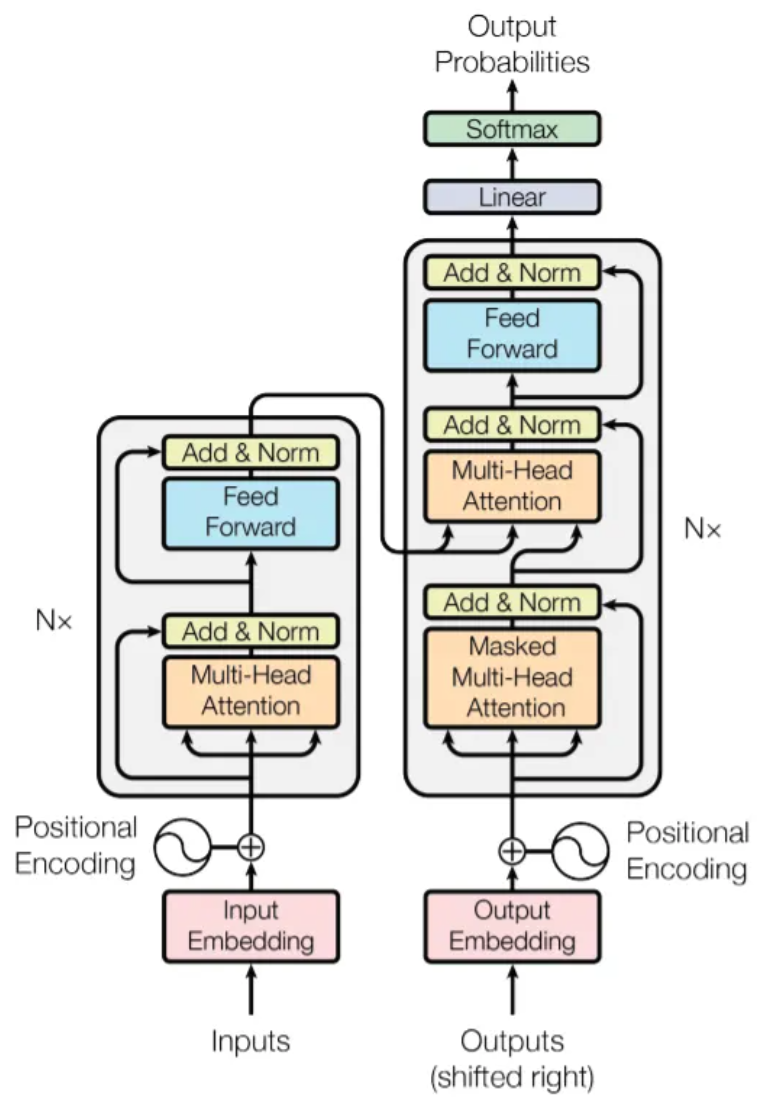
\includegraphics[width=0.5\textwidth]{../imgs/transformer.png}
      \end{figure}
\end{itemize}


\end{document}